\begin{frame}
    \frametitle{Cyclus vs. Unified Database: Total Spent Fuel Mass}
    General Conclusion: Cyclus simulation overpredicts total spent fuel mass 
    before 2000 and underpredicts total spent fuel mass after 2000. 

    \begin{figure}[htbp!]
      \begin{center}
        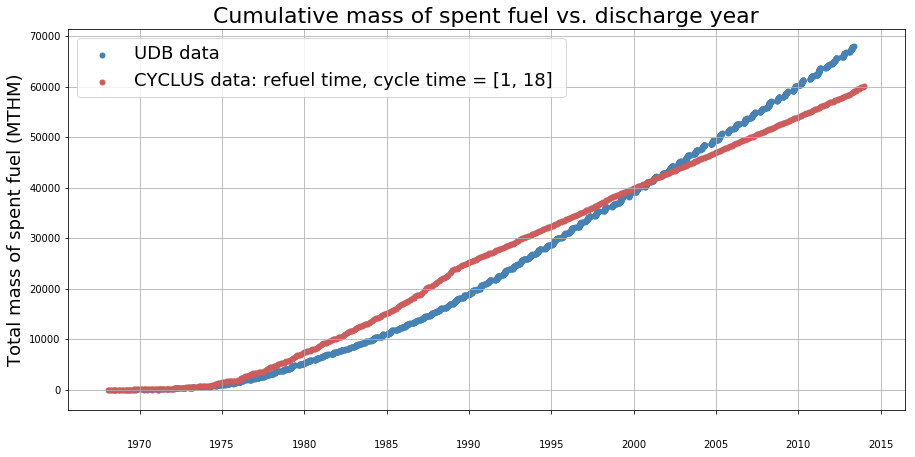
\includegraphics[height=5cm]{../figures/cumulative_mass_udb_cyclus}
      \end{center}
            \caption{The cumulative spent fuel mass against discharge time
            for Cyclus and Unified Database data from 1968 through 2013.}
      \label{fig:totalmass}
    \end{figure}

  \end{frame}

\begin{frame}
    \frametitle{Varying Refueling durations in Cyclus Simulation}
    General Conclusions: Longer reactor refueling durations shifts Cyclus simulation results closer to 
    UDB results before the year 2000. 
    \begin{figure}[htbp!]
        \begin{center}
          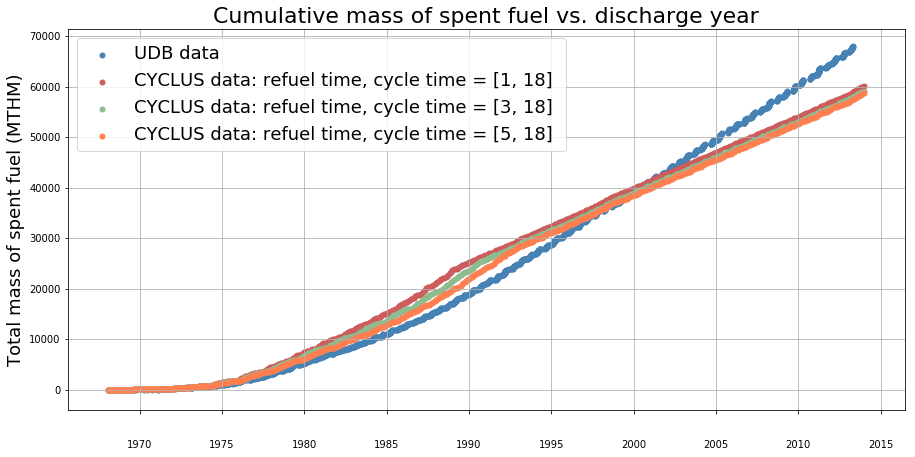
\includegraphics[height=5cm]{../figures/cumulative_mass_udb_cyclus_refueltime}
        \end{center}
        \caption{The cumulative spent fuel mass against discharge time
        for Cyclus and Unified Database data from 1968 through 2013 for varying
        \textbf{refueling durations}.}
    \end{figure}  
\end{frame}

\begin{frame}
  \frametitle{Varying Cycle durations in Cyclus Simulation}
  General Conclusions: Shorter reactor cycle lengths shifts Cyclus simulation results closer to 
    UDB results after the year 2000. 
  \begin{figure}[htbp!]
      \begin{center}
        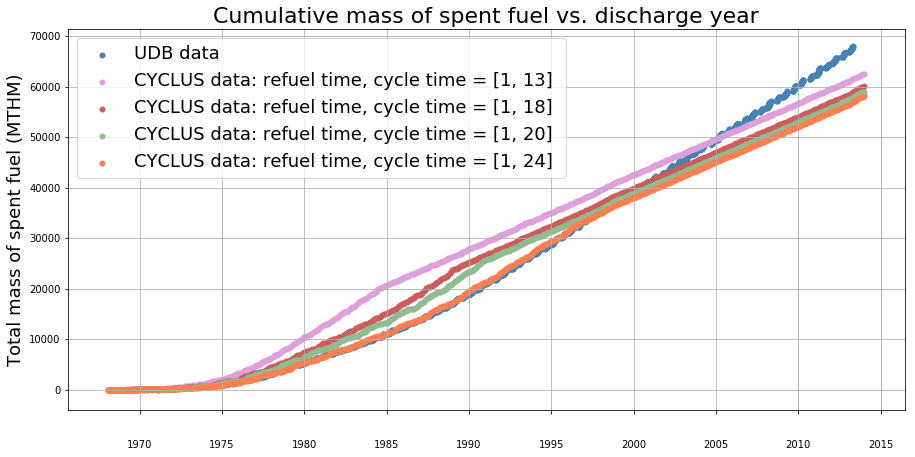
\includegraphics[height=5cm]{../figures/cumulative_mass_udb_cyclus_cycletime}
      \end{center}
      \caption{The cumulative spent fuel mass against discharge time
      for Cyclus and Unified Database data from 1968 through 2013 for varying
      \textbf{cycle durations}.}
  \end{figure}  
\end{frame}